\chapter{پیاده‌سازی، آزمایش‌ها و ارزیابی}\label{chap4}
\minitoc
\section{مقدمه}
تا به حال به لحاظ نظری به نحوه حل مسئله پرداخته شد. در این فصل پس از معرفی دادگان آموزشی و معیارهای ارزیابی مورد استفاده، نحوه پیاده‌سازی و دشواری‌های پیش‌آمده هنگام آموزش شرح داده خواهند شد. در انتها نیز ضمن گزارش نتایج، عملکرد مدل‌ها با یکدیگر مقایسه شده‌اند.
\section{دادگان آموزشی} \label{chap4:dataset}
\bff{\lr{Stanford Sentiment Treebank (SST)}}:
این دادگان حاوی حدود ۱۱ هزار نظر مثبت و منفی راجع به فیلم‌ها است \cite{sst}. به مانند سایر مدل‌ها جملات با طول کمتر از ۲۵ کلمه انتخاب شد که باقی مانده، ۲۲۰۷ جمله مثبت و منفی دادگان آموزشی، ۹۴۶ جمله دادگان \validation{} و ۱۳۵۰ جمله دادگان آزمون با اندازه واژگان ۷۴۷۹ خواهد بود.
\\
\bff{\lr{Yelp Restaurant (Yelp)}}:
این دادگان حاوی حدود ۶۰ هزار نظر مثبت و منفی کاربران راجع به رستوران‌ها است که زیرمجموعه‌ای از دادگان اصلی است
\LTRfootnote{\url{https://www.yelp.com}}.
حداکثر طول این جملات ۳۰ و با اندازه واژگان ۷۸۰۲، ۴۵ هزار داده آموزشی، ۵ هزار جمله \validation{} و ۱۰ هزار جمله دادگان آزمون است.
\\
\bff{\lr{Amazon Application-Book Review (Amazon)}}:
این دادگان حاوی حدود ۲۲۰ هزار نظر کاربران راجع به کتاب و یا برنامه‌های موجود در فروشگاه \lr{Amazon} است که زیرمجموعه‌ای از دادگان اصلی است \cite{amazon_review}. در واقع این دادگان بر خلاف دو دادگان دیگر، دارای شروط مثبت و منفی نبوده و شروط آن موضوع نظر که شامل کتاب یا برنامه است، می‌باشد. حداکثر طول این جملات ۴۰ و اندازه واژگان ۶۲۸۲ بوده و شامل 174622 داده آموزشی، 19402 جمله \validation{} و 19436 داده آزمون است.
\\
لازم به ذکر است در تمامی دادگان فوق، تعداد داده‌های شروط مختلف یکسان است.
\section{معیارهای ارزیابی} \label{chap4:metrics}
در ابتدا لازم است تا متذکر شد، از آنجا که در مدل‌های با فضای نهان امکان محاسبه دقیق \likelihood{} وجود ندارد، این معیار از معیارهای ارزیابی حذف گردیده است. به عنوان جایگزین از معیار‌های مبتنی \ngramphrase{} استفاده خواهد شد.
\subsection{\bleu{}}
معروف‌ترین معیار مبتنی بر \ngramphrase{} معیار \bleu{} است. این معیار در اصل در حوزه ترجمه ماشین معرفی شده است و کاربرد فراگیری دارد. این معیار که
\trans{\correlation{}}{Correlation}
آن با قضاوت انسانی تایید شده است \cite{bleu}، بر اساس مشابهت \ngramphrase{} جملات ترجمه شده تولیدی با جملات ترجمه موجود در دادگان آزمون است. از آنجا که برای یک جمله چندین ترجمه وجود دارد، به میزانی که \ngramphrase{}‌های جمله تولیدی با تعداد بیشتری از مجموعه \ngram{}‌های جملات ترجمه شده مرجع (آزمون)‌همخوانی داشته باشد، مدل امتیاز بالا‌تری خواهد گرفت. لازم به ذکر است که خروجی این معیار عددی بین صفر و یک بوده و اعداد بالاتر نشان دهنده کیفیت بالاتر جمله ترجمه شده است \cite{bleu}.
\\
این روش ارزیابی در حوزه تولید متن نیز بسیار کاربرد دارد. از آنجا که در تولید متن، مفهوم جمله مبدأ و مقصد وجود ندارد تا شباهت با جمله مقصد مقایسه شود، همه دادگان آزمون به عنوان مجموعه مرجع فرض خواهد شد و شباهت تک تک جملات تولید شده با مجموعه آزمون اندازه‌گیری و گزارش می‌شود \cite{seqgan}.
\\
نکته منفی این معیار، حساس نبودن آن به تنوع جملات است. از آنجا که شباهت هر جمله تولیدی مستقل از سایر جملات ارزیابی می‌شود، حتی اگر مدل تعداد زیادی جمله یکسان اما با کیفیت تولید نماید، عدد بالایی به مدل اختصاص خواهد یافت و این موضوع مطلوب نیست \cite{jointly}.
\\
لازم به ذکر است که در این معیار و تمامی دیگر معیارهای مبتنی بر \ngramphrase{}، حداکثر طول \ngramphrase{} مشخص است. برای مثال اگر حدااکثر طول \ngramphrase{} در نظر گرفته شده ۲ باشد، به به آن \bleu[-2]{} گفته می‌شود.
\subsection{\selfbleu{}}
این معیار نیز بسیار به لحاظ محاسباتی شبیه معیار \bleu{} است اما حساس به تنوع جملات تولیدی و غیر حساس به کیفیت جملات است. در این معیار، شباهت هر جمله با سایر جملات تولیدی اندازه‌گیری می‌شود؛ واضح است که هر اندازه شباهت جملات به یکدیگر کمتر باشد، از نظر این معیار امتیاز بهتری کسب خواهد کرد. به طور دقیق‌تر شباهت \bleu{} هر جمله با در نظر گرفتن سایر جملات به عنوان مجموعه مرجع، معیار \selfbleu{} خواهد بود \cite{seqgan}. همان طور که از شرح معیار بر‌می‌آید، این معیار کیفیت جملات را در نظر نگرفته و تنها شباهت جملات تولیدی به یکدیگر و یا به عبارت دیگر تنوع جملات را اندازه‌گیری می‌کند \cite{jointly}. لازم به ذکر است که مدل با نمونه‌ها متنوع عددی نزدیک به صفر و مدل با نمونه‌های تنوع کم عددی نزدیک به یک کسب خواهد کرد.
\subsection{\jaccard{}}
از آنجا که دو معیار \bleu{} و \selfbleu{} هر کدام به تنهایی به ترتیب ارزیابی‌گر کیفیت و تنوع هستند، معیار دیگری به نام \jaccard{} وجود دارد که ترکیب کیفیت و تنوع را در نظر می‌گیرد \cite{jointly}. این معیار بر خلاف \bleu{} که هر جمله را مستقل از سایر جملات تولیدی با مجموعه مرجع مقایسه می‌کرد، شاخصه‌های کل مجموعه تولیدی را با شاخصه‌هایی از کل مجموعه مرجع (آزمون)‌مقایسه می‌کند که این شاخصه تعداد تکرار هر \ngramphrase{} است. بنابراین اگر شاخصه‌ای از مجموعه تولیدی با مجموعه مرجع، چه به دلیل عدم رعایت کیفیت و چه عدم رعایت تنوع همخوانی نداشته باشد، از نظر این معیار جریمه خواهد شد \cite{jointly}.
\subsection{درصد رعایت شرط}
معیارهای معرفی شده تا به حال، کیفیت و تنوع جملات را مستقل از شرط بررسی می‌کردند. برای بررسی مدل‌ها از این جهت نیز می‌توان از یک \classifier{} قدرتمند بهره برد
\cite{toward, sentigan}؛
به این صورت که برای مثال اگر شرط با دو مقدار مثبت و منفی داشته باشیم، تعدادی برچسب مثبت و منفی اولیه در نظر گرفته؛ توسط مدل، جملات با مقدار شروط متناظر تولید نموده و در نهایت برچسب این جملات توسط \classifier{} تعیین نمود. درصد تطابق برچسب‌های \classifier{} با برچسب‌های اولیه دقت در رعایت شرط خواهد بود
\cite{toward, sentigan}.
در مقالات گذشته به دلیل معرفی نشدن مدل‌های \pretrain{} شده عظیم همچون \lr{BERT} از \classifier{}های دیگری استفاده می‌شد. این شبکه‌ها با
\trans{\finetuning{}}{Fine-tuning}
بر روی \task{}‌های مختلف، در بسیاری از \task{}ها موفق به کسب \stateoftheart{} شده‌اند \cite{bert}. اما نکته این دسته از مدل‌ها حجم زیاد آن‌هاست. بارگذاری  این مدل‌ها در \gpu{} و \finetuning{} آن‌ها به حافظه زیادی نیاز است. به همین هدف مدل‌های دیگری با اندازه کوچکتر با امکان بارگذاری در \gpu{}‌ در دسترس عموم، امکان \finetuning{} را فراهم کرده‌اند. نسخه کم حجم شده \lr{BERT}،
\lr{DistilBERT}
نام دارد که در دادگان \lr{SST} دقت ۹۴ درصد برای آن گزارش شده است \cite{distilbert}. با استفاده از این شبکه و \finetuning{} آن بر روی هر دادگان به طور مجزا به درصد دقت‌های ۸۷، ۹۷ و ۹۹ در به ترتیب دادگان \sst{}، \yelp{} و \amazon{} رسیده شد.
\iffalse
	می‌توان به عنوان جایگزین از معیارهایی همچون \revperplexity{} استفاده نمود. این روش به این صورت است که یک مدل زبانی میانی با استفاده از نمونه‌های مدل آموزش داده شده و \likelihood{} نمونه‌های آموزشی در مدل آموزش داده شده اندازه‌گیری می‌شود. این معیار نیز حساس به کیفیت و تنوع است. اگر مدل میانی آموزش داده شده، چه به دلیل عدم تنوع  و یا عدم کیفیت نمونه‌های مدل مورد ارزیابی احتمال کمی به نمونه‌های آموزشی نسبت دهد، معیار حساس بوده و مدل را جریمه خواهد کرد. نکته قابل توجه این است که به دلیل اینکه معیار آموزش مدل میانی، بر اساس بیشینه کردن \likelihood{} است، این امکان وجود دارد تا مدل مورد آموزش رفتار \meanseeking{} از خود بروز داده و به نقاطی که نمونه آموزشی از آن‌ها وجود ندارد، احتمال بالایی نسبت دهد. اما این اتفاق زمانی رخ می‌دهد که ظرفیت مدل کمتر از پیچیدگی نمونه‌های آموزشی باشد؛ این در حالیست که این نمونه‌های آموزشی توسط مدل مشابهی با ظرفیت مشابه تولید شده اند و احتمالا چنین نگرانی‌ای وجود نخواهد داشت.
\fi
\section{آموزش مدل}
همان طور که در فصل \ref{chap3} توضیح داده شد، آموزش شبکه از دو بخش کلی تشکیل شده است. اولین بخش مربوط به آموزش \wae{} است. به این منظور از معماری \transformer{}در \encoder{} و \decoder{} با بردارهای  \embedding{}
۱۲۸ تایی و فضای نهان ۵۱۲ بُعدی استفاده شد. لازم به ذکر است که ۴ خروجی اولِ لایه آخر \encoder{} به عنوان بردار فضای نهان به کار بسته شده است. نتایج با سایر معماری‌ها نیز گزاش شده‌ است. برای مولد شرطی نیز از دو لایه \lr{MAF} که هر لایه آن شامل سه لایه \lr{MADE} است بهره برده شده است. طبیعتا اندازه ورودی و خروجی این شبکه نیز ۵۱۲ بُعدی خواهد بود.
\\
همان طور که در بخش \ref{chap3:wae_training} توضیح داده شد، \decoder{} بایستی
$G(Z) = \argmax_{x} P_\psi(x|Z)$
و فضای خروجی $P_\psi$ یک بردار $|V|^{m}$ بعدی است که $m$ حداکثر طول جملات و $|V|$ نیز اندازه واژگان است؛ اما از آنجا که توانایی محاسباتی یافتن $\argmax$ بر روی چنین فضای بزرگی را نداریم بنابراین از روش
\trans{\greedydecoding{}}{Greedy decoding}
که تقریبی از $\argmax$ بر روی کل فضاست استفاده می‌کنیم.

\subsubsection{معماری‌های متفاوت در \encoder{} و \decoder{}}
به منظور بررسی اثر معماری‌های مختلف بر آموزش یک \wae{}، حالت‌های مختلف مورد آزمایش قرار گرفت. از دو معماری قدرتمند \lstm{} و \transformer{} در \decoder{} و سه معماری \lstm{}، \cnn{}  و \transformer{} در \encoder{} استفاده شده و نتایج در شکل \ref{fig:chap4:archs} آمده است. لازم به ذکر است که تعداد پارامتر‌های معماری‌های مختلف تقریبا نزدیک به یکدیگر بوده و اندازه \embedding{} کلمات با یکدیگر یکسان در نظر گرفته شده است.

\begin{figure}[h]
	\centering
	\begin{subfigure}{0.3\textheight}
		\centering
		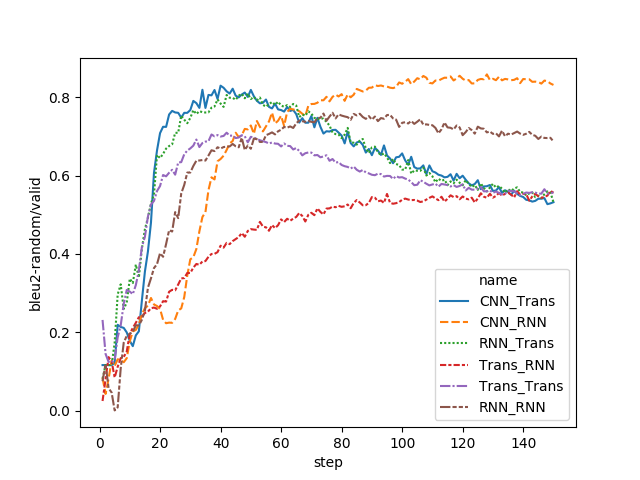
\includegraphics[width=1.\textwidth]{images/figs/bleu2-random.png}
		\caption{کارایی مدل‌های مختلف بر اساس معیار \bleu[-2]{}}
		\label{fig:chap4:archs_bleu}
	\end{subfigure}
	\begin{subfigure}{0.3\textheight}
		\centering
		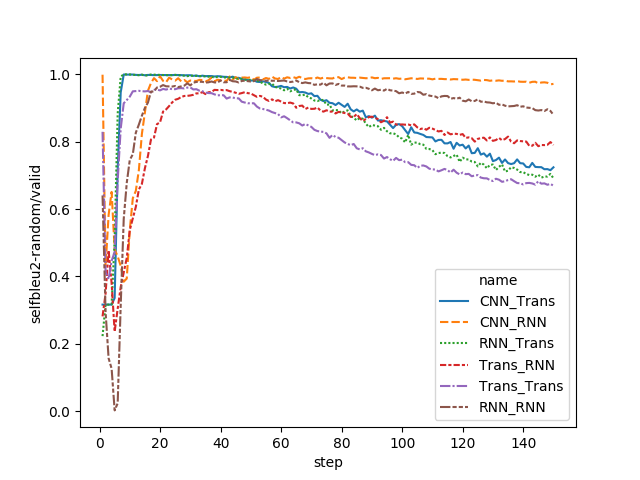
\includegraphics[width=1.\textwidth]{images/figs/selfbleu2-random.png}
		\caption{کارایی مدل‌های مختلف بر اساس معیار \selfbleu[-2]{}}
		\label{fig:chap4:archs_selfbleu}
	\end{subfigure}
	\begin{subfigure}{0.3\textheight}
		\centering
		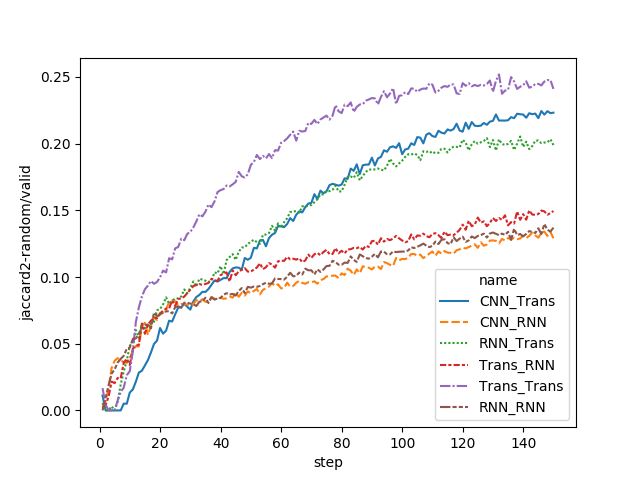
\includegraphics[width=1.\textwidth]{images/figs/jaccard2-random.png}
		\caption{کارایی مدل‌های مختلف بر اساس معیار \jaccard[-2]{}}
		\label{fig:chap4:archs_jac}
	\end{subfigure}
	\begin{subfigure}{0.3\textheight}
		\centering
		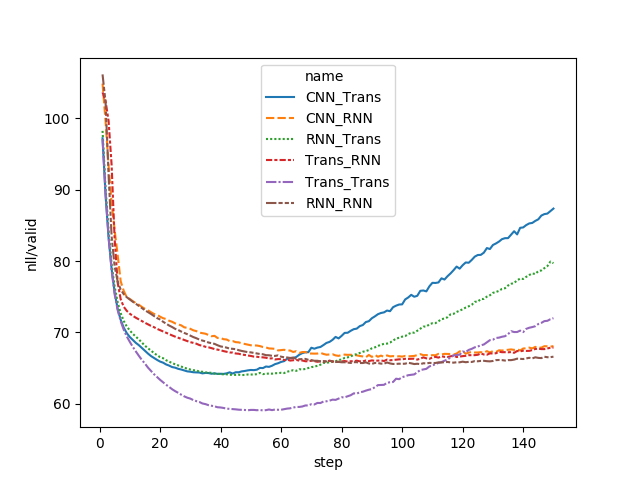
\includegraphics[width=1.\textwidth]{images/figs/nll.png}
		\caption{
			کارایی مدل‌های مختلف بر اساس معیار خطای بازسازی (منفی لگاریتم \likelihood{} باز‌سازی جمله)}
		\label{fig:chap4:archs_nll}
	\end{subfigure}
	\caption{
		کارایی معماری‌های مختلف در معیارهای \bleu[-2]{}، \selfbleu[-2]{}، \jaccard[-2]{} و خطای بازسازی.
		نام \lr{x-y} به معنای آن است که در \encoder{} از معماری x و در \decoder{} معماری y استفاده شده است. محور افقی تعداد \lr{epoch} است.}
	\label{fig:chap4:archs}
\end{figure}

همان طور که در شکل \ref{fig:chap4:archs_bleu} مشخص است، بهترین مدل بر اساس معیار \bleu[-2]{}، مدل \lr{CNN-RNN} است؛ اما میزان تاثیر فضای نهان بر خروجی \decoder{} چقدر است؟ به این منظور از معیار \selfbleu[-2]{} استفاده شده است. همان طور که در \ref{fig:chap4:archs_selfbleu} قابل رؤیت است، \selfbleu[-2]{} معماری \lr{CNN-RNN} عددی نزدیک به یک دارد؛ به این معنی که جملات تولید شده توسط این مدل، شباهت زیادی به یکدیگر دارند. بنابراین چنین مدلی مطلوب ما نخواهد بود. برای مقایسه همزمان این دو معیار از دو معیار دیگر \jaccard[-2]{} و خطای بازسازی استفاده نمودیم. همان طور که در شکل \ref{fig:chap4:archs_jac} مشخص است، بهترین مدل بر اساس این معیار، معماری \lr{Trans-Trnas} به معنای استفاده از معماری \transformer{} در \encoder{} و \decoder{}، است. از سوی دیگر کمینه مقدار خطای بازسازی طبق شکل \ref{fig:chap4:archs_nll} و همچنین متنوع‌ترین نمونه‌ها با توجه به معیار \selfbleu[-2]{} نیز اختصاص به همین مدل یافته است. بنابراین، معماری \transformer{} در این \task{} از سایر معماری‌ها موفق‌تر عمل کرده برای آزمایشات بعدی مورد استفاده قرار خواهد گرفت. در مورد سایر معماری‌ها نیز این طور باید گفت که مدل‌های دارای \transformer{} در \decoder{} دارای تنوع و \jaccard[-2]{} بالاتری هستند.
\iffalse
	\subsection{\encoder{}،
		عامل آموزش ناموفق}
	پس از آموزش شبکه توضیح داده شده، معضل عدم توجه \decoder{} به فضای نهان پیش آمد. تصاویر ؟؟؟ مربوط به نتایج \bleu{} و \selfbleu{} در دو حالت گزارش شده است. در حالت اول یک مجموعه جمله از دادگان
	\trans{\validation{}}{Validation}
	به فضای نهان برده شده و مجددا بازسازی ‌شده و \bleu{} و \selfbleu{} این مجموعه نسبت به داده آزمون اندازه‌گیری و گزارش شده است. این حالت را حالت بازسازی می‌نامیم. در حالت دوم تعدادی نمونه از \priordist{} گرفته شده و توسط \decoder{}
	\decode{}
	شده و مجددا معیارهای ذکر شده گزارش شده‌اند. این حالت را نیز حالت نمونه‌برداری می‌نامیم.
	مقادیر \bleu{} و \selfbleu{} دادگان \validation{} بر روی دادگان آزمون نیز به شرح زیر است:
	عکس بلو سلف بلو :)
	اعداد بلو سلف بلوی دیتا :)
	\\
	همان طور که در تصاویر ؟؟؟ مشخص است، با اینکه مقدار \bleu{} از دادگان اصلی بیشتر است (!) اما \selfbleu{} نزدیک به یک است! این موضوع نشان از این دارد که به ازای تغییرات $z$ در فضای نهان، خروجی \decoder{} تغییر چندانی نمی‌کند. مشاهده نمونه‌های تولید شده توسط مدل نیز گواهی بر این موضوع است.
	گواه موضوع :)
	\\
	حدس اولیه بر این بود که اتفاقی شبیه به آنچه در \vae{} گزارش شده است، رخ داده است. به منظور آزمایش دقیق‌تر یک \autoencoder{} ساده و بدون هیچ تابع هزینه اضافی آموزش داده شد. نتایج به شرح زیر بدست آمد:
	نتایج به شرح :)
	\\
	به وضوح مشخص است که پدیده مشابهی رخ داده است. بنابراین مشکل احتمالا از نحوه آموزش نیست. در گام بعدی تغییر معماری در \encoder{} و \decoder{} مورد بررسی قرار گرفت. معماری‌های مورد آزمایش \lr{LSTM}، \lr{CNN} و \lr{Transformer}  بودند. از آنجا که قدرت \lr{CNN} در تولید جمله در مقایسه با \lr{LSTM} کمتر است، از بررسی \lr{CNN} به عنوان \decoder{} صرف نظر شد. لازم به ذکر است که به دلیل اعمال نکردن توزیعی بر فضای نهان، اعداد برای حالت بازسازی گزارش شده‌اند.
	عکس معماری‌های متفاوت و ترکیبشان :)
	\\
	نکته قابل توجه این است که گویا مشکل در معماری \encoder{} نهفته است. در صورت استفاده از معماری \transformer{} مشکل عدم توجه به فضای نهان تقریبا رفع شده و \bleu{} و \selfbleu{} در حالت بازسازی تقریبا برابر با مقادیر این معیار برای دادگان \validation{} است. نکته قابل توجه دیگر این است که معماری \lstm{} و \transformer{} در \decoder{} تفاوت چندانی ایجاد نمی‌کند و تنها مسیر حرکت متفاوتی دارند.
	به دلیل همگرایی سریع‌تر معماری \transformer{}، این معماری برای سایر آزمایشات برگزیده شد. در ادامه با استفاده از معماری \transformer{} یک \wae{} آموزش داده شد که نتایج به شرح زیر است:
	شرح آزمایش :)
	\\
\fi
\iffalse
	\subsection{استفاده از  \gan{} به جای \mmd{}}
	در بخش‌های متفاوتی صحبت از رفتار \modecollapse{}
	\gan{}
	سخن به میان آمد. در اینجا طی یک آزمایش از \lr{WGAN} به جای \mmd{} برای یادگیری فضای نهان یک \autoencoder{} استفاده شد. به عبارت دیگر اگر $F(\epsilon)$ شبکه‌ای باشد که با گرفتن یک نوفه با توزیع گاوسی نرمال، آن را به نمونه‌ای در فضای نهان تبدیل کند و $D(Z)$ یک \critic{} بین نمونه‌های تولید شده توسط $F$ و فضای نهان ساخته شده توسط \encoder{}
	$Q(Z|X)$
	باشد، تابع هزینه ذیل استفاده گشت:
	\begin{gather}
		\mathcal{L}_\text{WGAN} (F, D)=
		\expected_{x \sim P_\text{Data}(X), z \sim Q(Z|x)} D(z)
		- \expected_{\epsilon \sim N(\bff{0}, \bff{I}), z \sim F(\epsilon)} D(z)
		\\
		\text{\lr{s.t: D is 1-Lipschitz}} \nonumber
	\end{gather}
	که نسبت به $D$ بیشینه و نسبت به $F$ کمینه می‌گردد. برای برآوردن شرط \lr{1-Lipschitz} بودن $D$ نیز از روش \lr{Gradient Penalty} استفاده شده است. اگر $\bff{z}$ و $\tilde{\bff{z}}$ به ترتیب نمونه‌هایی از $Q$ و $F$ ،
	$t$
	متغیر تصادفی از توزیع یکنواخت $[0,1]$ و
	$\hat{z} = t\bff{z} + (1 - t) \tilde{\bff{z}}$
	باشد، \lr{Gradient Penalty} به صورت زیر نوشته می‌شود \cite{wgan_gp}:
	\begin{gather}
		\mathcal{L}_\text{WGAN-GP} (D; \bff{z}, \tilde{\bff{z}}) = \lambda_{gp} \expected_{t \sim U(0, 1)}
		(|| \nabla_{\hat{\bff{z}}} D(\hat{\bff{z}}) ||_2  - 1)^2
	\end{gather}
	که در کنار تابع هزینه اصلی بهینه‌سازی می‌شود. نتایج آزمایش فوق به شرح زیر است:
	شرح آزمایش :)
	\\
\fi
\iffalse
	\section{آموزش مولد شرطی}
\fi

\subsubsection{نمودار‌های آموزش \wae{} و مولد شرطی}
نمودارهای مربوط به آموزش \wae{} و مولد شرطی با دادگان \amazon{} به ترتیب در شکل‌های \ref{fig:chap4:amazon_cond} و \ref{fig:chap4:amazon_flow} آمده است. کم شدن تابع هزینه در \ref{fig:chap4:amazon_enc_cls} را می‌توان به میزان دسته‌بندی شدن جملات در فضای نهان نسبت به مقادیر شرط و افزایش معیار \jaccard{} در شکل \ref{fig:chap4:amazon_flow_jaccard} را به یادگیری مطلوب فضای نهان توسط شبکه مولد، تعبیر نمود.
\begin{figure}[H]
	\centering
	\begin{subfigure}{0.3\textheight}
		\centering
		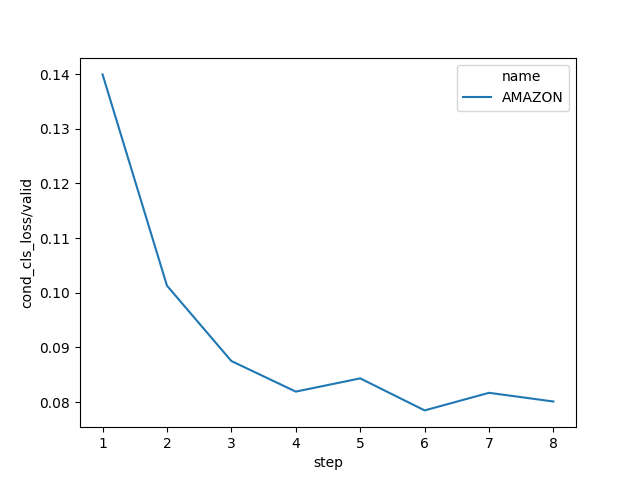
\includegraphics[width=1.\textwidth]{images/figs/2020_01_03__19_09_40__cond_cls_loss.png}
		\caption{}
		\label{fig:chap4:amazon_enc_cls}
	\end{subfigure}
	\begin{subfigure}{0.3\textheight}
		\centering
		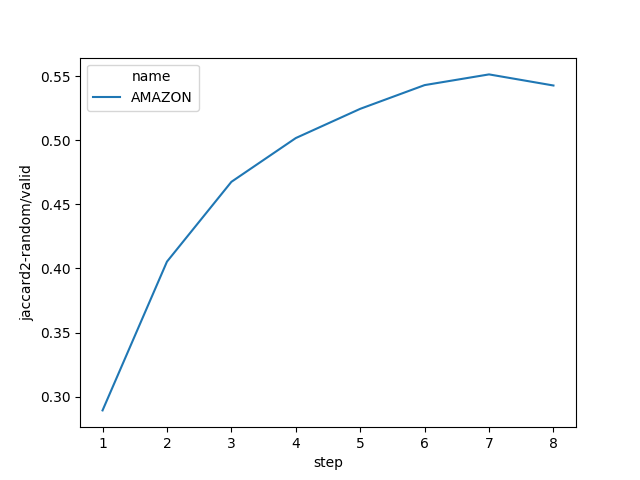
\includegraphics[width=1.\textwidth]{images/figs/2020_01_03__19_09_40__jaccard2-random.png}
		\caption{}
		\label{fig:chap4:amazon_jaccard}
	\end{subfigure}
	\begin{subfigure}{0.3\textheight}
		\centering
		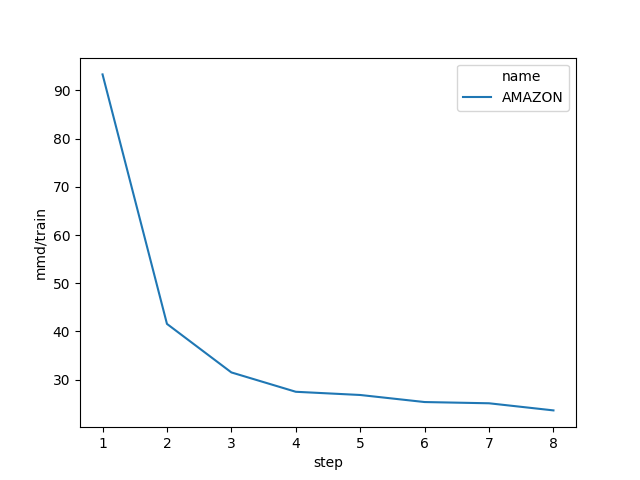
\includegraphics[width=1.\textwidth]{images/figs/2020_01_03__19_09_40__mmd.png}
		\caption{}
		\label{fig:chap4:amazon_mmd}
	\end{subfigure}
	\begin{subfigure}{0.3\textheight}
		\centering
		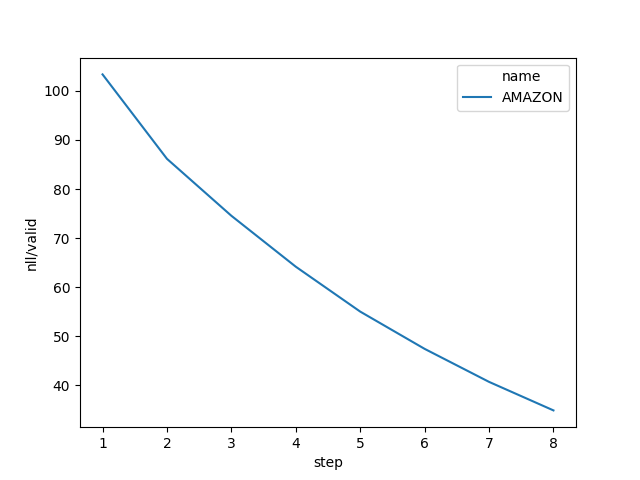
\includegraphics[width=1.\textwidth]{images/figs/2020_01_03__19_09_40__nll.png}
		\caption{}
		\label{fig:chap4:amazon_nll}
	\end{subfigure}
	\caption{
		نمودار‌های آموزش \wae{} بر روی دادگان \amazon{}.
		هزینه دسته‌بندی بردار‌های نهان تولید شده توسط \encoder{}
		(\subref{fig:chap4:amazon_enc_cls})؛
		کیفیت و تنوع جملات تولیدی با توجه به معیار \jaccard{}
		(\subref{fig:chap4:amazon_jaccard})؛
		فاصله توزیع \marginal{} \encoder{} و \priordist{} با توجه به معیار \mmd{}
		(\subref{fig:chap4:amazon_mmd})؛
		خطای بازسازی جملات
		(\subref{fig:chap4:amazon_nll}).
	}
	\label{fig:chap4:amazon_cond}
\end{figure}
\newpage
\begin{figure}[h]
	\centering
	\begin{subfigure}{0.3\textheight}
		\centering
		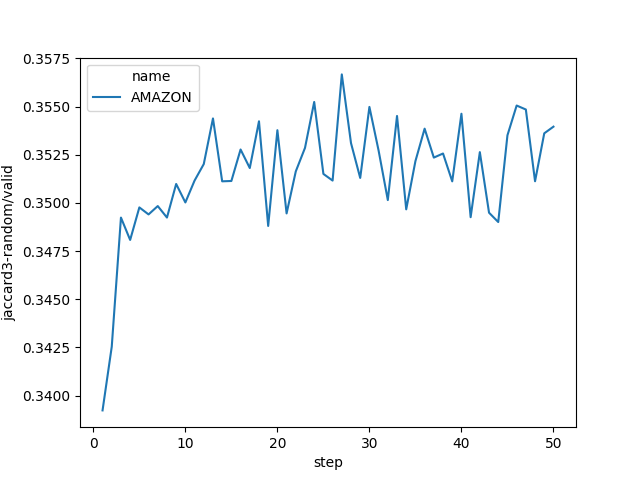
\includegraphics[width=1.\textwidth]{images/figs/2020_01_03__19_13_00__jaccard3-random.png}
		\caption{}
		\label{fig:chap4:amazon_flow_jaccard}
	\end{subfigure}
	\begin{subfigure}{0.3\textheight}
		\centering
		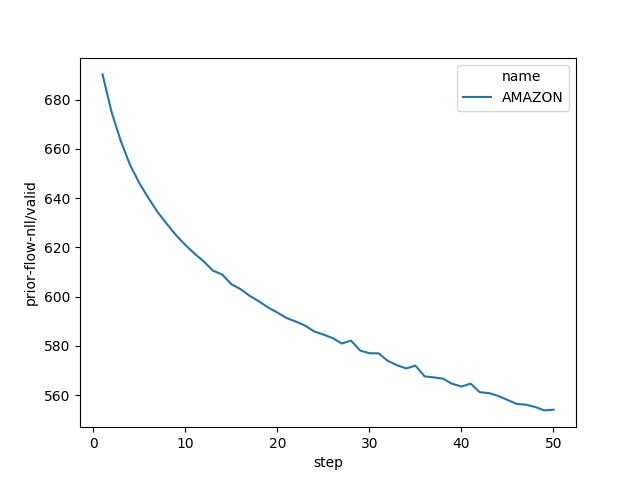
\includegraphics[width=1.\textwidth]{images/figs/2020_01_03__19_13_00__prior-flow-nll.png}
		\caption{}
		\label{fig:chap4:amazon_flow_nll}
	\end{subfigure}
	\caption{
		نمودار‌های آموزش مولد شرطی بر روی دادگان \amazon{}.
		کیفیت و تنوع جملات تولیدی تولید شده توسط مدل مولد شرطی با توجه به معیار \jaccard{}
		(\subref{fig:chap4:amazon_flow_jaccard})؛
		تابع هزینه آموزش مولد شرطی
		(\subref{fig:chap4:amazon_flow_nll}).
	}
	\label{fig:chap4:amazon_flow}
\end{figure}

\section{نتایج و مقایسه با سایر مدل‌ها}
از بین مدل‌های شرطی ذکر شده، مدل‌های ساده به دلیل سادگی حذف و مدل \lr{CSGAN} نیز به دلیل ارائه نکردن کد پیاده‌سازی حذف شدند. بنابراین مدل‌های پایه شامل دو مدل \towardctg{} و \sentigan{} هستند اولی بر پایه \vae{} و دیگری بر پایه \gan{} است. در تمامی آموزش‌ها و برای تمامی مدل‌ها، اندازه بردار \embedding{} کلمات و فضای نهان مدل‌ها ۱۲۸ و بردار فضای نهان خروجی \encoder{}، ۵۱۲ در نظر گرفته شده است. در مورد معماری \encoder{} و \decoder{} نیز از معماری \transformer{} استفاده شده است.
\\
همان طور که در بخش \ref{chap4:dataset} توضیح داده شد، مدل‌ها بر روی دادگان آموزشی \lr{SST} آموزش داده شده و سپس بر اساس معیارهای  دقت رعایت شرط، \bleu{} ، \selfbleu{} و \jaccard{} مورد ارزیابی قرار گرفته‌اند. نتایج در جدول \ref{table:mr15_result} گزارش شده است.
\begin{table*}[!htb]
	\centering
	\caption{
		ارزیابی مدل‌های پایه و ارائه شده آموزش داده شده بر روی دادگان \lr{AmazonAppBook}، بر اساس معیار‌های مختلف}
	\label{table:amazon_result}
	\small\tabcolsep=0.07cm
	\begin{tabular}{||c||c c c|c c|c c|c c||}\hline\hline نام مدل & AC0                        & AC1                        & Total AC                   & BL2                        & BL5                        & SBL2                       & SBL5                       & JAC2                       & JAC5                       \\
		\hline\hline
		waerandenccond2                                & $0.968$                    & $0.971$                    & $0.969$                    & $0.907$                    & $0.310$                    & $0.919$                    & $\cellcolor{gray!25}0.371$ & $\cellcolor{gray!25}0.651$ & $\cellcolor{gray!25}0.247$ \\
		\hline
		waedisentangle                                 & $\cellcolor{gray!25}0.999$ & $\cellcolor{gray!25}0.999$ & $\cellcolor{gray!25}0.999$ & $\cellcolor{gray!25}0.943$ & $0.426$                    & $0.948$                    & $0.568$                    & $0.537$                    & $0.219$                    \\
		\hline
		newtoward0.8ctextgen                           & $0.983$                    & $0.980$                    & $0.982$                    & $0.928$                    & $\cellcolor{gray!25}0.444$ & $0.894$                    & $0.469$                    & $0.457$                    & $0.223$                    \\
		\hline
		senti                                          & $0.991$                    & $0.996$                    & $0.994$                    & $0.903$                    & $0.422$                    & $\cellcolor{gray!25}0.892$ & $0.468$                    & $0.539$                    & $0.237$                    \\
		\hline
		\hline\end{tabular}\normalsize
\end{table*}

\begin{table*}[!htb]
	\centering
	\caption{
		ارزیابی مدل‌های پایه و ارائه شده آموزش داده شده بر روی دادگان \lr{YelpRestaurant}، بر اساس معیار‌های مختلف}
	\label{table:yelp_result}
	\small\tabcolsep=0.07cm
	\begin{tabular}{||c||c c c|c c|c c|c c||}\hline\hline نام مدل & AC0                        & AC1                        & Total AC                   & BL2                        & BL5                        & SBL2                       & SBL5                       & JAC2                       & JAC5                       \\
		\hline\hline
		waerandenccond2                                & $0.810$                    & $0.964$                    & $0.887$                    & $0.686$                    & $0.155$                    & $\cellcolor{gray!25}0.753$ & $\cellcolor{gray!25}0.186$ & $0.462$                    & $0.102$                    \\
		\hline
		waedisentangle                                 & $\cellcolor{gray!25}0.965$ & $\cellcolor{gray!25}0.991$ & $\cellcolor{gray!25}0.978$ & $0.799$                    & $0.231$                    & $0.868$                    & $0.351$                    & $0.416$                    & $0.116$                    \\
		\hline
		newtoward0.8ctextgen                           & $0.892$                    & $0.933$                    & $0.912$                    & $0.765$                    & $0.232$                    & $0.802$                    & $0.310$                    & $\cellcolor{gray!25}0.489$ & $\cellcolor{gray!25}0.141$ \\
		\hline
		senti                                          & $0.942$                    & $0.987$                    & $0.965$                    & $\cellcolor{gray!25}0.807$ & $\cellcolor{gray!25}0.302$ & $0.834$                    & $0.467$                    & $0.338$                    & $0.093$                    \\
		\hline
		\hline\end{tabular}\normalsize
\end{table*}

همان طور که در جداول \ref{table:amazon_result} و \ref{table:yelp_result} مشخص است، عملکرد مدل پیشنهادی با اینکه در درصد رعایت شرط از مدل \sentigan{} عقب‌تر است اما از مدل مشابه فضای‌نهان‌دار \towardctg{} بهتر است. از حیث کیفیت و تنوع نیز در \jaccard[-2]{} از سایرین عملکرد بهتری داشته و در \jaccard[-5]{} نیز در دادگان \amazon{} از مدل \towardctg{} موفق‌تر بوده است.
\\
\iffalse
نکته قابل توجه و قابل بحث، اختلاف بیشتر درصد رعایت شرطِ مدل پیشنهادی از مدل \towardctg{} در دادگان \amazon{} است. علت این موضوع را شاید این طور بتوان جست‌وجو کرد که دادگان \amazon{} از دو موضوع تشکیل شده است؛ کتاب و برنامه. این دو موضوع چندان فضای مفهومی مشترکی ندارند؛ در حالی که دادگان \yelp{} همگی در مورد غذا و رستوران هستند. از این رو منطقی به نظر می‌رسد برای مدل اول فضای نهان $\bff{Z}$ تماما توسط شرط تعیین شود در حالی که در دادگان دیگر، مفاهیم و شرط می‌توانند مستقل از هم بوده و هر دو با هم یک جمله را تعیین کنند. مدل گرافی این دو دیدگاه در شکل \ref{fig:chap4:dataset_pgm} آمده است.
\begin{figure}[h]
	\centering
	\begin{subfigure}{0.1\textheight}
		\centering
		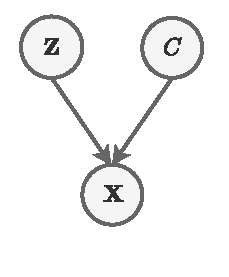
\includegraphics[width=1.\textwidth]{images/pgm_disentangle.pdf}
		\caption{}
		\label{fig:chap4:dataset_pgm_d}
	\end{subfigure}
	\hspace{1cm}
	\begin{subfigure}{0.2\textheight}
		\centering
		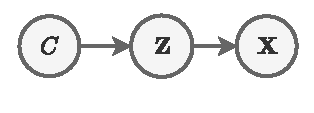
\includegraphics[width=1.\textwidth]{images/pgm_hierarchical.pdf}
		\caption{}
		\label{fig:chap4:dataset_pgm_h}
	\end{subfigure}
	\caption{
		دو مدل گرافی متفاوتی که می‌توان برای یک \task{} شرطی در نظر گرفت.
		فضای نهان و شرط مستقل از هم
		(\subref{fig:chap4:dataset_pgm_d}، دادگان \yelp{})؛
		شرط به طور کامل فضای نهان را تعیین می‌کند
		(\subref{fig:chap4:dataset_pgm_h}، دادگان \amazon{}).
	}
	\label{fig:chap4:dataset_pgm}
\end{figure}
با در نظر گرفتن این توضیحات، به دلیل آنکه مدل \towardctg{} به نوعی استقلال بین شرط و فضای نهان $\bff{Z}$ را ایجاد می‌کند، چندان همخوانی با ذات دادگان \amazon{} نداشته و عملکرد ضعیف‌تری را از خود نشان می‌دهد.
\fi

\begin{table*}[!htb]
    \centering
	\caption{
    ارزیابی مدل‌های پایه و ارائه شده آموزش داده شده بر روی دادگان \lr{SST}، بر اساس معیار‌های مختلف}
\label{table:mr15_result}
    \small\tabcolsep=0.07cm
    \begin{tabular}{||c||c c c|c c|c c|c c||}\hline\hline نام مدل	& AC0	& AC1	& Total AC	& BL2	& BL5	& SBL2	& SBL5	& JAC2	& JAC5\\
        \hline\hline
        waerandenccond2	& $0.641$	& $0.807$	& $0.724$	& $0.588$	& $0.114$	& $\cellcolor{gray!25}0.783$	& $\cellcolor{gray!25}0.238$	& $0.252$	& $0.036$ \\
        \hline
        waedisentangle	& $0.797$	& $0.873$	& $0.835$	& $0.553$	& $0.104$	& $0.805$	& $0.296$	& $0.224$	& $0.028$ \\
        \hline
        newtoward0.8ctextgen	& $0.487$	& $0.800$	& $0.644$	& $\cellcolor{gray!25}0.628$	& $\cellcolor{gray!25}0.171$	& $0.792$	& $0.508$	& $\cellcolor{gray!25}0.263$	& $\cellcolor{gray!25}0.045$ \\
        \hline
        senti	& $\cellcolor{gray!25}0.827$	& $\cellcolor{gray!25}0.919$	& $\cellcolor{gray!25}0.873$	& $0.583$	& $0.155$	& $0.799$	& $0.587$	& $0.228$	& $0.035$ \\
        \hline
        \hline\end{tabular}\normalsize 
\end{table*}


اما در مورد دادگان \sst{}، همان طور که در جدول \ref{table:mr15_result} مشخص است، مدل ارائه شده در دقت یکی از دسته‌ها از مدل مشابه مبتنی بر فضای نهانِ \towardctg{} بهتر عمل کرده است؛ این در حالیست که در دقت دسته دیگر، عملکرد ضعیف و در دقت کلی مانند روش \towardctg{} بوده است. در مورد \bleu{} و \selfbleu{} نیز از لحاظ تنوع عملکرد بهتری داشته است. برای مثال در مورد \bleu[-5]{} و \selfbleu[-5]{}، با اینکه \bleu{} تقریبا نزدیک به سایرین نگه داشته شده است اما \selfbleu{}ی آن عدد پایینی داشته و تنوع بیشتری دارد. لازم به ذکر است که علی‌رقم این موضوع، در معیار \jaccard{} که ترکیب کیفیت و تنوع را در نظر می‌گیرد، با اینکه بهترین عملکرد \jaccard[-2]{} را داشته اما در \jaccard[-5]{} با فاصله از سایر مدل‌ها قرار گرفته است.
\\
در مورد دلیل عملکرد ضعیف مدل پیشنهادی و همچنین \towardctg{} که هر دو مدل مبتنی بر فضای نهان هستند، باید گفت که احتمالا به دلیل کم بودن و از سوی دیگر پیچیده بودن آن، فضای نهان معنای متناسب با جملات را در خود نداشته و توابع هزینه‌ای که مبتنی بر معنای فضای نهان هستند به درستی عمل نمی‌کنند.
\\
در مورد موفق‌تر بودن مدل \sentigan{} نیز این طور می‌توان گفت که این مدل به ازای هر شرط یک مدل مولد مجزا در نظر گرفته است؛ بنابراین هر مولد وظیفه یادگیری بخش مربوط به خود را دارد؛ به عبارت دیگر مسئله شرطی را به صورت مسئله غیر شرطی حل کرده است و بنابراین احتمال رعایت نکردن شرط بسیار کمتر خواهد بود. فارغ از این موضوع، این مدل با افزایش تعداد شرط‌ها با مشکل مواجه خواهد شد.

\iffalse
	\subsubsection{بررسی رفتار مولد شرطی}
	به منظور بررسی رفتار مولد شرطی، یک آزمایش ترتیب داده شد. همان طور که پیش‌تر توضیح داده شد، علت تقسیم کردن فضای نهان با توجه به مقادیر مختلف شرط، کم بودن ظرفیت مولد شرطی و ضعف آن در یادگیری هر توزیع پیچیده‌ای بود. در اینجا نیز عملکرد نسبتا مناسب آن در یک دسته و عکس آن در دسته دیگر می‌تواند احتمالا به این موضوع مرتبط باشد. به این منظور در تابع هزینه آموزش مولد شرطی تغییر کوچکی اعمال شد؛ به جای اینکه احتمال هر نمونه با شرط مرتبطش را در مولد شرطی بیشینه کنیم، احتمال همان نقاط اما با مقدار شرط دیگری را کمینه میکنیم. در واقع از نقاط با برچسب شرط نادرست به عنوان نمونه منفی بهره گرفته و انتظار داریم مولد شرطی به نمونه‌های منفی احتمال کم اما به نمونه‌های مثبت احتمال بالایی نسبت دهد. به صورت صوری تابع هزینه ذیل به تابع هزینه اصلی افزوده می‌شود:
	\begin{align}
		\mathcal{L'}_c (F) = & \lambda_\text{neg} \expected_{c' \sim p_{C'\neq c}, \bff{x} \sim p_\text{Data}(\bff{X}|c), \bff{z} \sim q(\bff{Z}|\bff{x})} [\log p_F(\bff{z}|c')]
	\end{align}
	و تابع هزینه کلی به صورت زیر بدست می‌آید:
	\begin{align}
		\mathcal{L}_c (F) = & - \expected_{\bff{x} \sim p_\text{Data}(\bff{X}|c), \bff{z} \sim q(\bff{Z}|\bff{x})} [\log p_F(\bff{z}|\bff{c})] +                                 \\
		                    & \lambda_\text{neg} \expected_{c' \sim p_{C'\neq c}, \bff{x} \sim p_\text{Data}(\bff{X}|c), \bff{z} \sim q(\bff{Z}|\bff{x})} [\log p_F(\bff{z}|c')]
	\end{align}
	\begin{figure}[h]
		\centering
		\begin{subfigure}[t]{0.3\textheight}
			\centering
			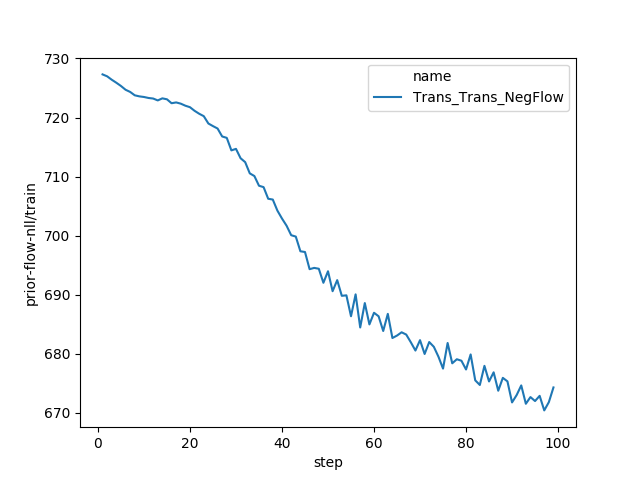
\includegraphics[width=1.\textwidth]{images/figs/2019_12_31__11_06_03__prior-flow-nll.png}
			\caption{}
			\label{fig:chap4:negprior_prior_nll}
		\end{subfigure}
		\begin{subfigure}[t]{0.3\textheight}
			\centering
			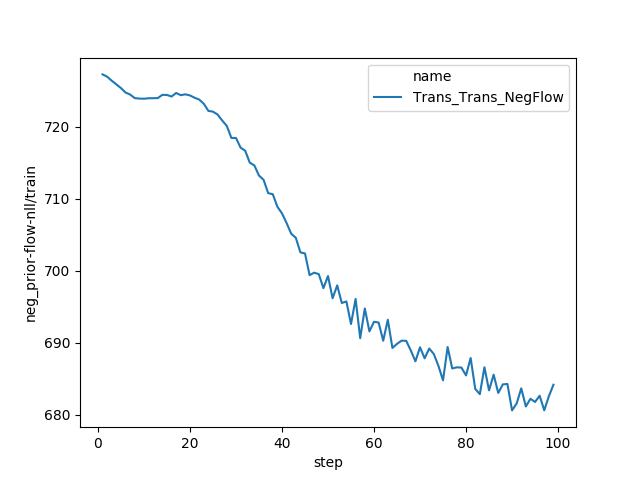
\includegraphics[width=1.\textwidth]{images/figs/2019_12_31__11_06_03__neg_prior-flow-nll.png}
			\caption{}
			\label{fig:chap4:negprior_negprior_nll}
		\end{subfigure}
		\caption{
			منفی لگاریتم \likelihood{} نمونه‌های مثبت (باید کمینه گردد)
			(\subref{fig:chap4:negprior_prior_nll}).
			منفی لگاریتم \likelihood{} نمونه‌های منفی (باید بیشینه گردد)
			(\subref{fig:chap4:negprior_negprior_nll}).
		}
		\label{fig:chap4:negprior}
	\end{figure}
	مطابق با شکل \ref{fig:chap4:negprior}، که نتیجه آموزش شبکه با توابع هزینه فوق با پارامتر
	$\lambda_\text{neg} = 0.05$
	است (با ضرایب بالاتر، آموزش ناپایدار می‌شد)، بر خلاف انتظارات، هر دو تابع با هم کمینه شدند. این موضوع به این معنی است که مدل مولد شرطی توانایی انتساب احتمال بالا به نمونه‌های مثبت و احتمال کم به نمونه‌های منفی را ندارد و یا هر دو کاهش می‌یابند و یا هر دو افزایش. از این مشاهده این طور می‌توان نتیجه‌گیری نمود که اعمال محدودیت تقسیم شده فضای نهان به مقادیر مختلف شرط، چندان کارساز نبوده و همچنان مولد شرطی توانایی تفکیک این دو دسته از یکدیگر را نداشته و احتمالا رفتار \meanseeking{} از خود بروز می‌دهد.
\fi

